%!TeX spellcheck = en-US
\documentclass{article}
\usepackage{enumerate}
\usepackage{amsmath}
\usepackage{amssymb}
\usepackage{graphicx}
\usepackage{subfigure}
\usepackage{geometry}
\usepackage{caption}
\usepackage{indentfirst}
\usepackage{array}
%\renewcommand\arraystretch{2}
\usepackage{tikz}
\usepackage{multicol}
\usepackage{algorithm}
\usepackage{algorithmicx}
\usepackage{algpseudocode}
\renewcommand{\algorithmicrequire}{\textbf{Input:}}
\renewcommand{\algorithmicensure}{\textbf{Output:}}
\usepackage{minted}
\usemintedstyle{autumn}
\geometry{left=3.0 cm,right=3.0 cm,top=3.0 cm,bottom=4.0 cm}
\renewcommand{\thesection}{Ex. \arabic{section}}
\title{VE281 Writing Assignment Five}
\author{Liu Yihao 515370910207}
\date{}

\begin{document}
\maketitle

\section{}
In Kruskal's algorithm, we take the shortest edge and connect two nodes if it doesn't form a cycle.
\begin{enumerate}
	\item Connect b and c
	\item Connect a and b
	\item Connect c and e
	\item Connect e and f
	\item Connect e and d
\end{enumerate}

The minimum spanning tree is
\begin{center}
	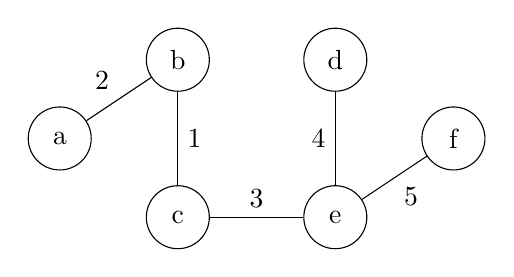
\begin{tikzpicture}
		\draw (-2.5,0) 	node (a) [draw,shape=circle,minimum size=0.8cm] {a};
		\draw (-1,1) 		node (b) [draw,shape=circle,minimum size=0.8cm] {b};
		\draw (-1,-1) 	node (c) [draw,shape=circle,minimum size=0.8cm] {c};
		\draw (1,1) 		node (d) [draw,shape=circle,minimum size=0.8cm] {d};
		\draw (1,-1) 		node (e) [draw,shape=circle,minimum size=0.8cm] {e};
		\draw (2.5,0) 	node (f) [draw,shape=circle,minimum size=0.8cm] {f};
		\draw (b) edge node [right] {1} (c);
		\draw (a) edge node [above left] {2} (b);
		\draw (c) edge node [above] {3} (e);
		\draw (e) edge node [below right] {5} (f);
		\draw (e) edge node [left] {4} (d);
	\end{tikzpicture}
\end{center}

\section{}
\begin{algorithm}[H]
	\begin{algorithmic}
		\Require \\
			A directed acyclic graph $G=(V,E)$ with real-valued edge weights \\
			Two distinct nodes $s$ and $d$
		\Ensure \\
			A longest weighted path from $s$ to $d$ if exists \\

		\State $L \gets G$ sorted in topological order
		\State Remove nodes located before $s$ or after $d$ from $L$
		\State Remove node $s$ from $L$
		\State $s.distance \gets 0$
		\State $s.predecessor \gets NULL$
		\For {node $v$ \textbf{in} $L$}
		\State $v.distance \gets -\infty$
		\State $v.predecessor \gets NULL$
			\For {edge $(u,v)$ \textbf{in} edges with end node $v$}
				\If {$u.distance + (u,v).weight > v.distance$}
					\State $v.distance \gets u.distance + (u,v).weight$
					\State $v.predecessor \gets u$
				\EndIf
			\EndFor
		\EndFor
		\If {$d.predecessor == NULL$}
			\State print ``No path exists"
		\Else
			\State print $d.predecessor$ recursively in reverse order
		\EndIf
	\end{algorithmic}
\end{algorithm}

The time complexity is $O(V+E)$.

\section{}
\begin{algorithm}[H]
	\begin{algorithmic}
		\Require \\
			A directed graph $G=(V,E)$ with real-valued edge reliability in the range $[0,1]$ \\
			Two distinct nodes $s$ and $d$
		\Ensure \\
			A most reliable path from $s$ to $d$ if exists \\

		\For {node $u$ \textbf{in} $G$}
			\State $u.reached \gets false$
			\State $u.probability \gets 0$
			\State $u.predecessor \gets NULL$
		\EndFor
		\State $s.probability \gets 1$
		\State push node $s$ into set $S$
		\While {Set $S$ is not empty}
			\State $u \gets$ pop the node with largest reliability in $S$
			\State $u.reached \gets true$
			\For {edge $(u,v)$ \textbf{in} edges with start node $u$}
				\If {\textbf{not} $v.reached$ \textbf{and} $u.probability * (u,v).reliability > v.probability $ }
					\State $v.probability \gets u.probability * (u,v).reliability$
					\State $v.predecessor \gets u$
				\EndIf
			\EndFor
		\EndWhile

		\If {$d.predecessor == NULL$}
			\State print ``No path exists"
		\Else
			\State print $d.predecessor$ recursively in reverse order
		\EndIf
	\end{algorithmic}
\end{algorithm}

\section{}
\begin{algorithm}[H]
	\begin{algorithmic}
		\Require \\
			A connected, undirected graph $G=(V,E)$
		\Ensure \\
			A path that traverses edge in E exactly once in each direction. \\

		\For {node $u$ \textbf{in} $G$}
			\State $u.reached \gets false$
			\State $u.depth \gets 0$
		\EndFor
		\State $s \gets$ an arbitrary node in $G$
		\State \Call {DFS}{$s$}
		\\
		\Function {DFS}{node $u$}
			\State $u.reached \gets true$
			\For {edge $(u,v)$ \textbf{in} edges adjacent to $u$}
				\If {\textbf{not} $v.reached$}
					\State $v.depth \gets u.depth + 1$
					\State traverse $u \to v$
					\State \Call {DFS}{$v$}
					\State traverse $v \to u$
				\ElsIf {$v.depth > u.depth$}
					\State traverse $u \to v$
					\State traverse $v \to u$
				\EndIf
			\EndFor
		\EndFunction

	\end{algorithmic}
\end{algorithm}

\section{}


\end{document}
